% Chapter 1

\chapter{Results and Analysis} % Main chapter title

\label{Chapter5} % For referencing the chapter elsewhere, use \ref{Chapter1} 

\lhead{Chapter 5. \emph{Results and Analysis}} % This is for the header on each page - perhaps a shortened title

\emph{In this section we present the results of our experimentation with feature engineering. We notably begin with a comparison between GROBID and refextract, the existing partial solution for metadata extraction at INSPIRE-HEP. Following this we detail our evaluation method and approach to running experiments. Finally, we present the results of our experimentation and provide our analysis and interpretations.}

\section{Comparison with \emph{refextract}}

As a first result for GROBID, we compare it with \emph{refextract}, the existing solution for automatic reference extraction at CERN. \emph{refextract} is an example of a \emph{stylistic analysis} tool (see Section \ref{sec:solutionmethods}), as it employs regular expressions in a heuristic framework for extraction. As previously mentioned, \emph{refextract} is incomplete and greatly lacking in both breadth and depth of detail. It is capable only of retrieving references\footnote{A comparatively easy task; GROBID's citation model usually performs at a significantly higher accuracy than, say, its \emph{header} model.}, and the classification itself is quite basic. Since the modelling of reference fields differs between the two, a comparison is difficult to make. Our results will at least be indicative, however, and we are able to make reasonable comparisons on the most important fields. The dataset for the comparison consists of 60 articles coming from the SCOAP$^3$ online repository\footnote{Scoap$^3$ (Sponsoring Open Consortium for Open Access Publishing in Particle Physics) is an open access digital library hosted at CERN, backed by an international partnership of research institutions.}.

Unlike \emph{refextract}, GROBID requires two separate models to classify the citations of a given article: the \emph{reference-segmenter} and \emph{citation} models\footnote{Strictly speaking, there is another model, (full) \emph{segmentation}, above the \emph{reference-segmenter}, and so \emph{citation} accuracy depends on this also. But because one focus of our work is to improve this model, we accept this omission.}. The \emph{reference-segmenter} model is the simplest model in GROBID's arsenal, and is responsible for segmenting a reference list block into individual references. Therefore, the accuracy of the citation model is ultimately subject to the accuracy of the reference block inputs supplied to it by the \emph{reference-segmenter} above. The results for training and evaluating the \emph{reference-segmenter} on 60 SCOAP$^3$ papers with an 80--20 split are given in Table \ref{table:referencesegmenterresults}. The results show the \emph{reference-segmenter} is extremely accurate. In fact, only 5 token misclassifications out of 622 were made for the <label> class, and from a grand total of 12,981.

\label{subsec:refextract}
\begin{table}[h]
\begin{center}
\begin{tabular}{|c|cccc|}
\hline
label           & accuracy  & precision  & recall   & f1 \\
\hline
<label>         & 99.96     & 100        & 99.2     & 99.6\\
<reference>     & 99.96     & 99.96      & 100      & 99.98\\
\hline
(micro average) & 99.96     & 99.96      & 99.96    & 99.96  \\
(macro average) & 99.96     & 99.98      & 99.6     & 99.79  \\
\hline
\end{tabular}
\caption[Evaluation results for reference segmentation]{Evaluation results for reference segmentation}
\label{table:referencesegmenterresults}
\end{center}
\end{table}

The most significant difference between the tools is the set of classes modelled. \emph{refextract} attempts only to classify to the minimum detail required for identifying the originating document within INSPIRE-HEP. Therefore, there are no equivalents to GROBID's classes, <volume>, <pages>, and so on. Rather, these parts of references are absorbed into other, higher-level classes, and are indicated by a dash (-) in the results table. Comparisons can be made, however on fields, <title>, <author>, <journal>, and <date>. There we see the superiority of GROBID over \emph{refextract}. Note that here the \emph{citation} model was not trained on the evaluation set, and in particular this may explain its dismal performance in precision for the date field, and recall for \emph{pubnum}. The dataset instances contained a recurring publication number that was almost uniformly misclassified by GROBID as a date. Notice that this is an example of a domain specificity of HEP papers. Had we trained on these papers, we could expect an improvement.

That \emph{refextract} has perfect recall in the given fields is due to the way the evaluation was conducted, namely...

For an explanation of the performance metrics, see Section \ref{sec:evaluation}.

\begin{table}[h]
\begin{center}
\begin{tabular}{|c|cccc|cccc|}
\hline
engine &  \multicolumn{4}{|c|}{GROBID} & \multicolumn{4}{c|}{\emph{refextract}}\\
\hline
label & accuracy & precision & recall & f1 & acc. & prec. & rec. & f1\\
\hline
<author>    & 99.85 &   99.68   &   99.75   &   99.72   & 98.33 &   100 &   92.22   &   95.95   \\
<title> &   99.59   &   98.87   &   99.25   &   99.06   & 94.89 &   100 &   71.75   &   83.55   \\
<journal>   & 98.84 &   88.87   &   93.98   &   91.35   & 97.12 &   100 &   46.78   &   63.74   \\
<volume>&   99.95   &   99.07   &   98.15   &   98.6    & -     &   -   &   -       &   -   \\
<issue> &   99.93   &   100     &   94.63   &   97.24   & -     &   -   &   -       &   -   \\
<pages> &   99.75   &   93.51   &   99.45   &   96.39   & -     &   -   &   -       &   -   \\
<date>  &   98.39   &   57.39   &   98.31   &   72.47   & 98.88 &   100 &   37.55   &   54.6    \\
<pubnum>&   98.71   &   100     &   12.96   &   22.95   & -     &   -   &   -       &   -   \\
<note>  &   99.4    &   43.75   &   35      &   38.89   & -     &   -   &   -       &   -   \\
<publisher>&99.81   &   63.46   &   94.29   &   75.86   & -     &   -   &   -       &   -   \\
<location>& 99.81   &   86.32   &   91.11   &   88.65   & -     &   -   &   -       &   -   \\
<institution>& 99.78&   25      &   25      &   25      & -     &   -   &   -       &   -   \\
<booktitle>&    98.7&   55.56   &   41.67   &   47.62   & -     &   -   &   -       &   -   \\
<web>   &   99.64   &   51.85   &   100     &   68.29   & -     &   -   &   -       &   -   \\
<editor>    &  99.93&   100     &46.67      &   63.64   & -     &   -   &   -       &   -   \\
<tech>  &   99.95   &   83.33   &   50      &   62.5    & -     &   -   &   -       &   -   \\
\hline
(micro average) & 99.5  &   93.63   &   94.77   &   94.19 & -    &   - &   -   &   -   \\
(macro average) & 99.5  &   77.92   &   73.76   &   71.76 & -    &   -  &   -   &   -   \\
\hline
\end{tabular}
\caption[Evaluation results for citations]{Evaluation results for citations}
\label{table:citationcomparison}
\end{center}
\end{table}

\section{Experiment Setup}
\label{sec:experimentsetup}
Here talk about k-fold, number of iterations, computing resources etc.

\section{Evaluation Method}

Accuracy is defined to be,

\begin{equation}
\text{Accuracy} = \frac{TP + TN}{TP + FN + FP + TN},
\label{eq:accuracy}
\end{equation}

that is, the proportion of correct classifications to total classifications, where TP is the number \emph{true positives}, the correctly predicted positive classes, where \emph{positive} indicates any given class; TN is the number of \emph{true negatives}, the correctly predicted \emph{negative} classes; FN is the number of \emph{false positives}, the incorrectly predicted positive classes; and TN is the number of \emph{true negatives}. Accuracy can be a misleading statistic when we have uneven representations of classes in the dataset. In the event that we have high bias on the number of negatives, we can achieve excellent accuracy simply by always predicting the negative class. For this reason, we consider other statistics too. \emph{Precision} is the proportion of positives correctly claimed, that is,

\begin{equation}
\text{Precision} = \frac{TP}{TP + FP}.
\label{eq:precision}
\end{equation}

\emph{Recall} is the proportion of positives correctly predicted to the total number of positive occurrences (equivalently, the accuracy over the positive class), that is,

\begin{equation}
\text{Recall} = \frac{TP}{TP + FN}.
\label{eq:recall}
\end{equation}

Notice that in the case described above, both precision and recall would be 0. The $F_1$ statistic is a common measure used to assess classifiers, and is defined as,

\begin{equation}
F_1 = \frac{2 \times \text{precision} \times \text{recall}}{\text{precision} + \text{recall}},
\label{eq:f1}
\end{equation}

that is, the harmonic mean of precision and recall (the ``1'' in $F_1$ indicates the two are evenly weighted). The $F_1$ statistic is a nice way of summarising both at once as it is simply the harmonic mean of the two. Furthermore, because of this, a large imbalance in recall and precision resuts in a lower $F_1$ score. It is necessary to be good in both precision and recall to have a good $F_1$ score; the harmonic mean of any data is always upper-bounded by its arithmetic mean

\subsection{Evaluation in Grobid}

In Grobid, evaluation is done at the token, field, and instance levels, that is, Grobid calculates the aforementioned statistics for individual token or words, and then for the classes themselves. Finally, it calculates the number of correct instances, that is, entire samples with no classification errors.

We supplement the Grobid evaluation output with a confusion matrix, and example of which is shown in Figure XX. Whereas the statistics allow us to compare one model to another, a confusion matrix can be used to see exactly which misclassifications are being made, which can in turn inform our feature engineering.

\begin{table}[h]
\begin{center}
\begin{tabular}{ | p{0.2\linewidth} | p{0.25\linewidth} | p{0.15\linewidth} | p{0.3\linewidth} |}
\hline
Feature Category & Variations & Models & Data\\
\hline
Baseline & - & Segmentation, header & CORA, CORA app. HEP, CORA + HEP, HEP, HEP app. CORA \\
\hline
Baseline & - & Header & HEP app. 1/3 CORA, HEP app. 2/3 CORA \\
\hline
Dictionaries & First order, Second order, Third order & Header & HEP app. 1/3 CORA, HEP app. 2/3 CORA \\
\hline
Dicts. + Stops & First order, Second order, Third order, Stops only & Header & HEP app. 1/3 CORA, HEP app. 2/3 CORA \\
\hline
Regularisation & $\sigma=0$, $\sigma=\exp\{-6\}$,$\sigma=\exp\{-5\}$,$\sigma=\exp\{-4\}$,$\sigma=\exp\{-3\}$, & Header & HEP app. 1/3 CORA, HEP app. 2/3 CORA \\
\hline
Token Extension & +5, +10, +15, +20 & Header & HEP app. 1/3 CORA, HEP app. 2/3 CORA \\
\hline
Block Size & Height, Width, Height \& Width, Area & Segmentation, Header & HEP \\
\hline
Levenshtein & $T_1 = 0.05$, Lev$\geq0.1$, Lev$\geq0.2$, Lev$\geq0.4$, Lev$\geq0.8$, Lev$\geq0.1 \& \geq0.4$ LevAll & Header & HEP \\
\hline
Character Classes & Binary, Decimal, Decimal only & Segmentation & HEP \\
\hline
\end{tabular}
\caption[Character classes used as features, along with the regular expressions used to count them.]{Character classes used as features, along with the regular expressions used to count them.}
\label{table:experiments}
\end{center}
\end{table}

\section{Results}

\subsection{Baseline}

\begin{figure}[h]
\center
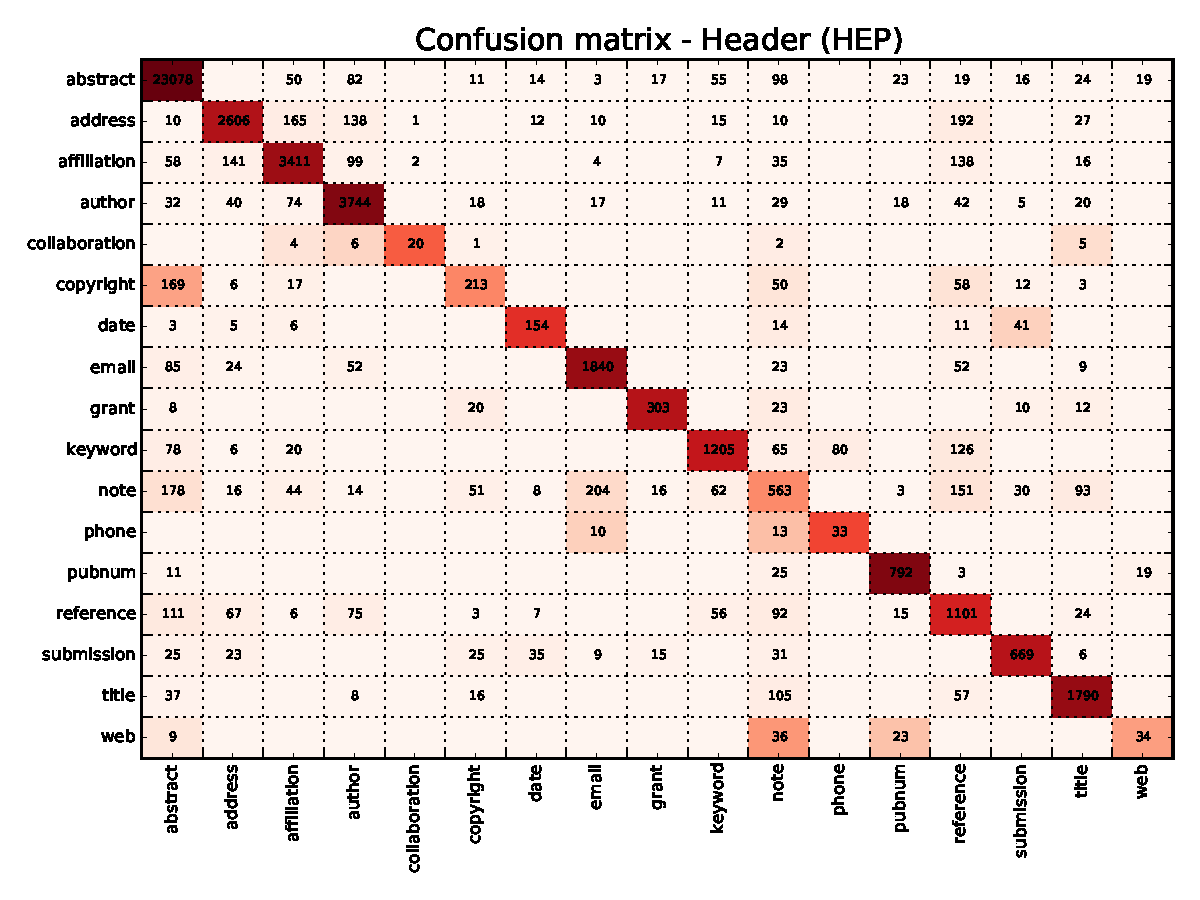
\includegraphics[width=5.5in]{Figures/header_baseline_confusion.pdf}
\caption{}
\label{fig:header_baseline_confusion}
\end{figure}

\begin{figure}[h]
\center
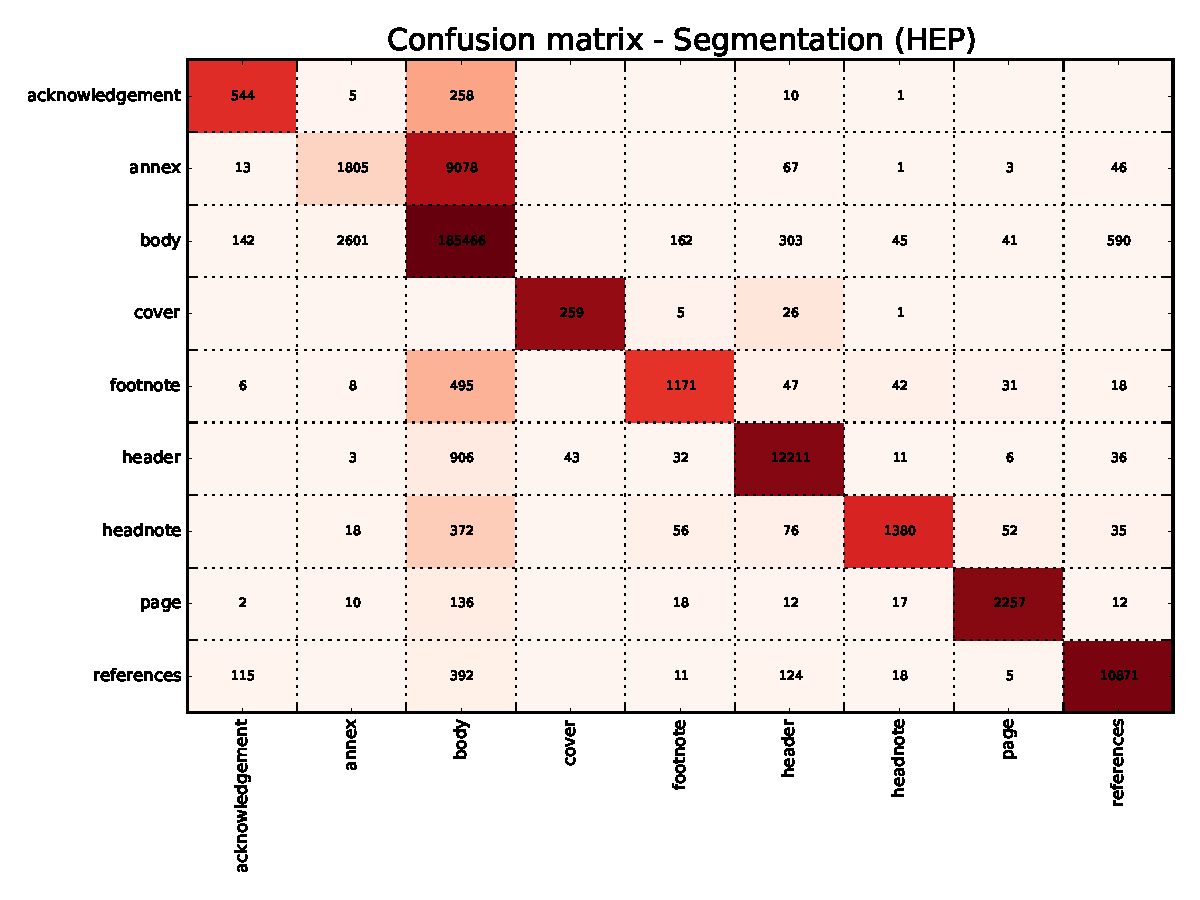
\includegraphics[width=5.5in]{Figures/segmentation_baseline_confusion.pdf}
\caption{}
\label{fig:segmentation_baseline_confusion}
\end{figure}

\subsection{Block Size}

\subsection{Character Classes}

\subsection{Dictionaries}

\subsection{Dictionaries + Stop Words}

\subsection{Levenshtein}

\subsection{Regularisation}

\subsection{Token Selection}

\subsection{Results Summary}

\begin{figure}[h]
\center
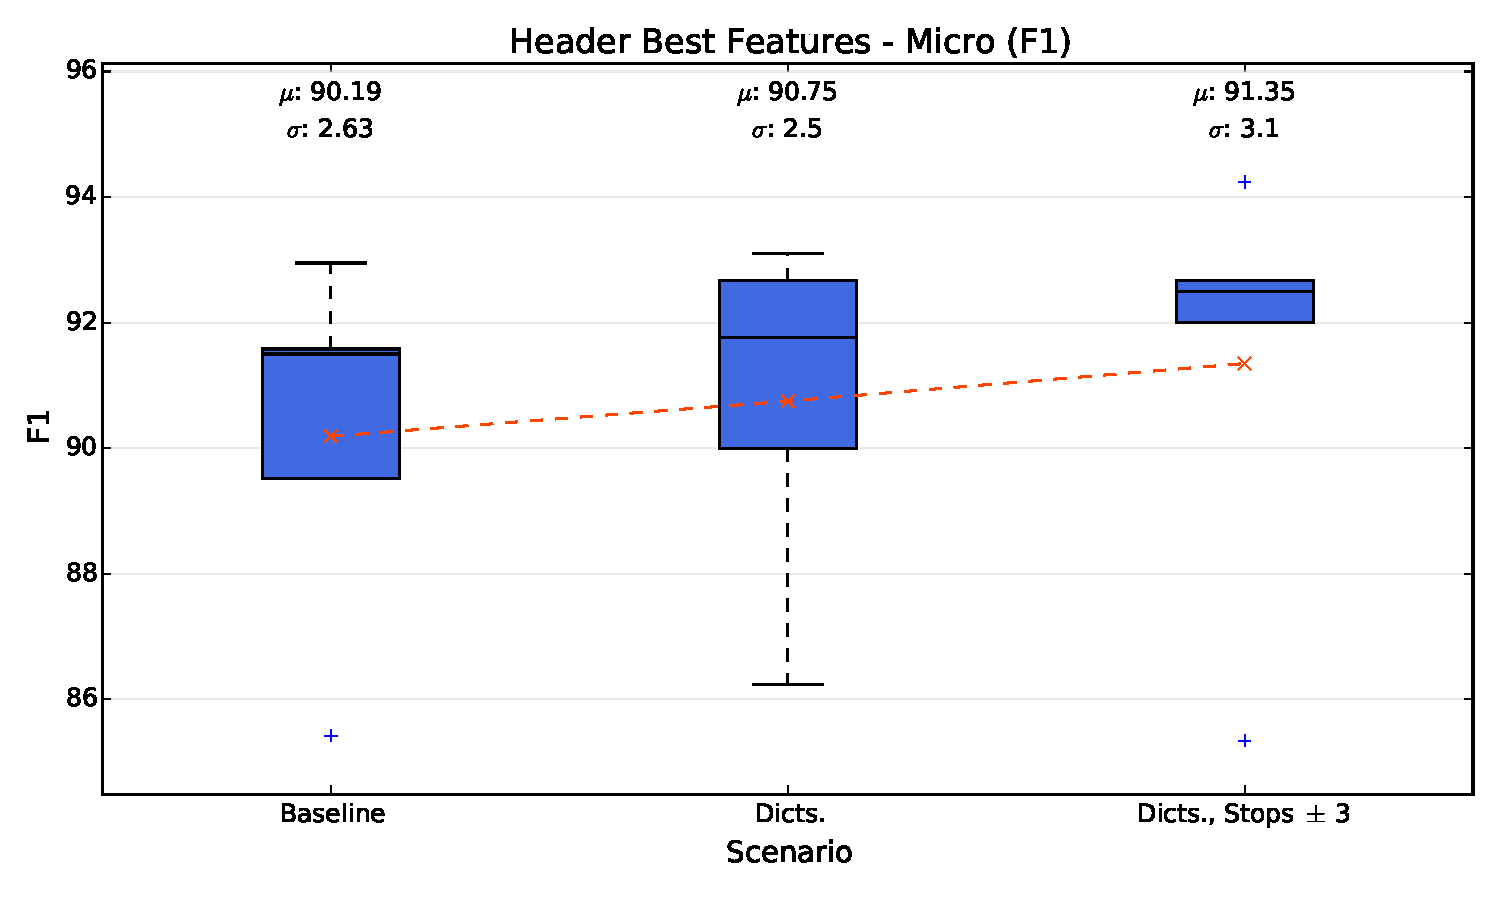
\includegraphics[width=5.5in]{Figures/micro.pdf}
\caption{}
\label{fig:micro}
\end{figure}

\begin{figure}[h]
\center
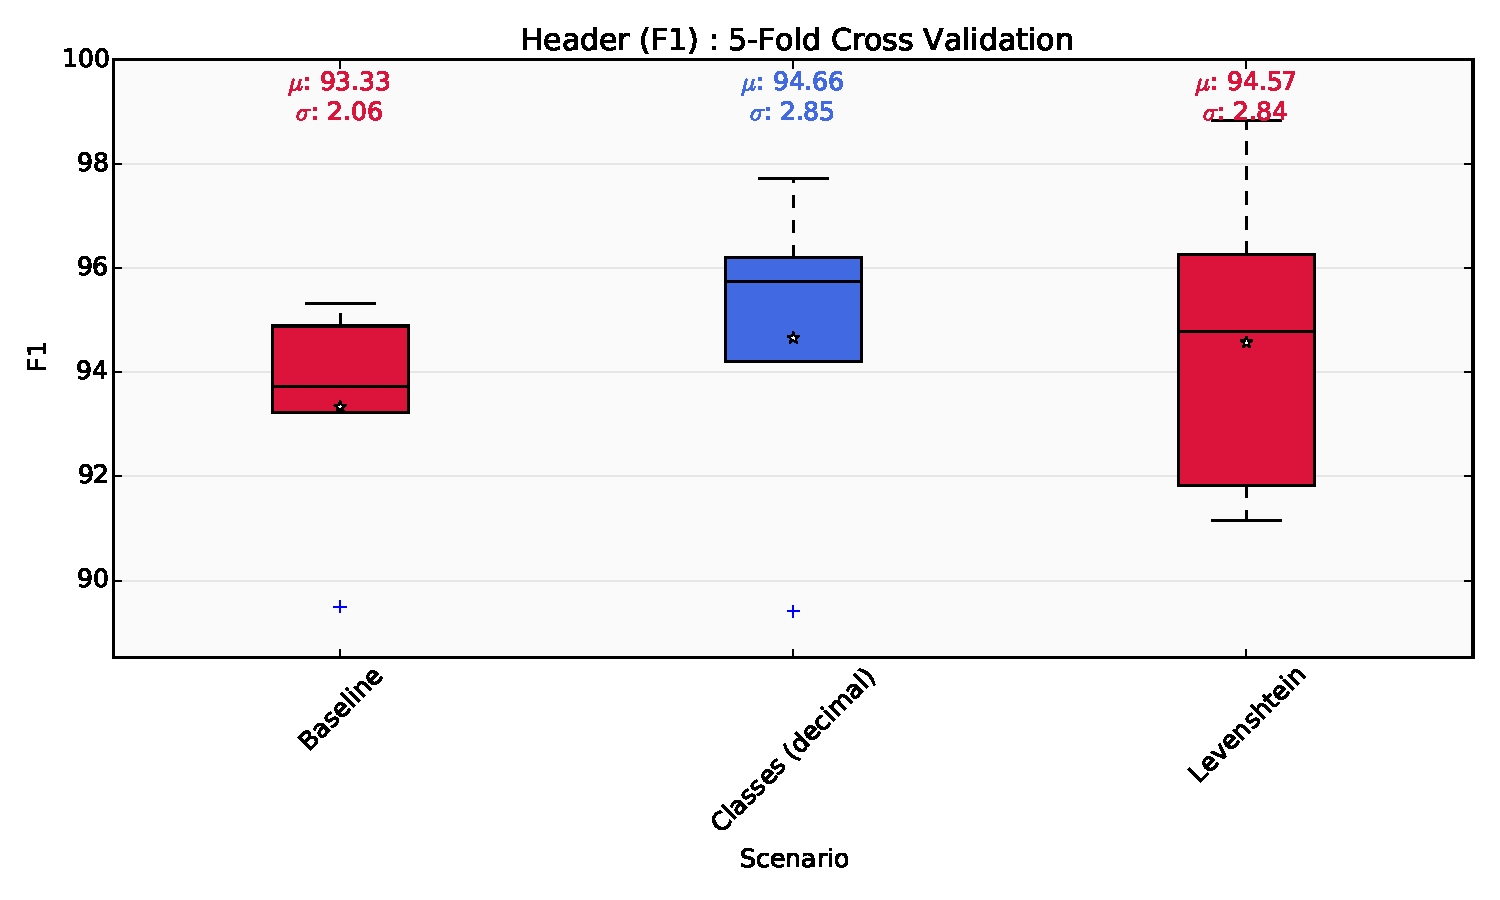
\includegraphics[width=5.5in]{Figures/header.pdf}
\caption{}
\label{fig:header}
\end{figure}

\begin{figure}[h]
\center
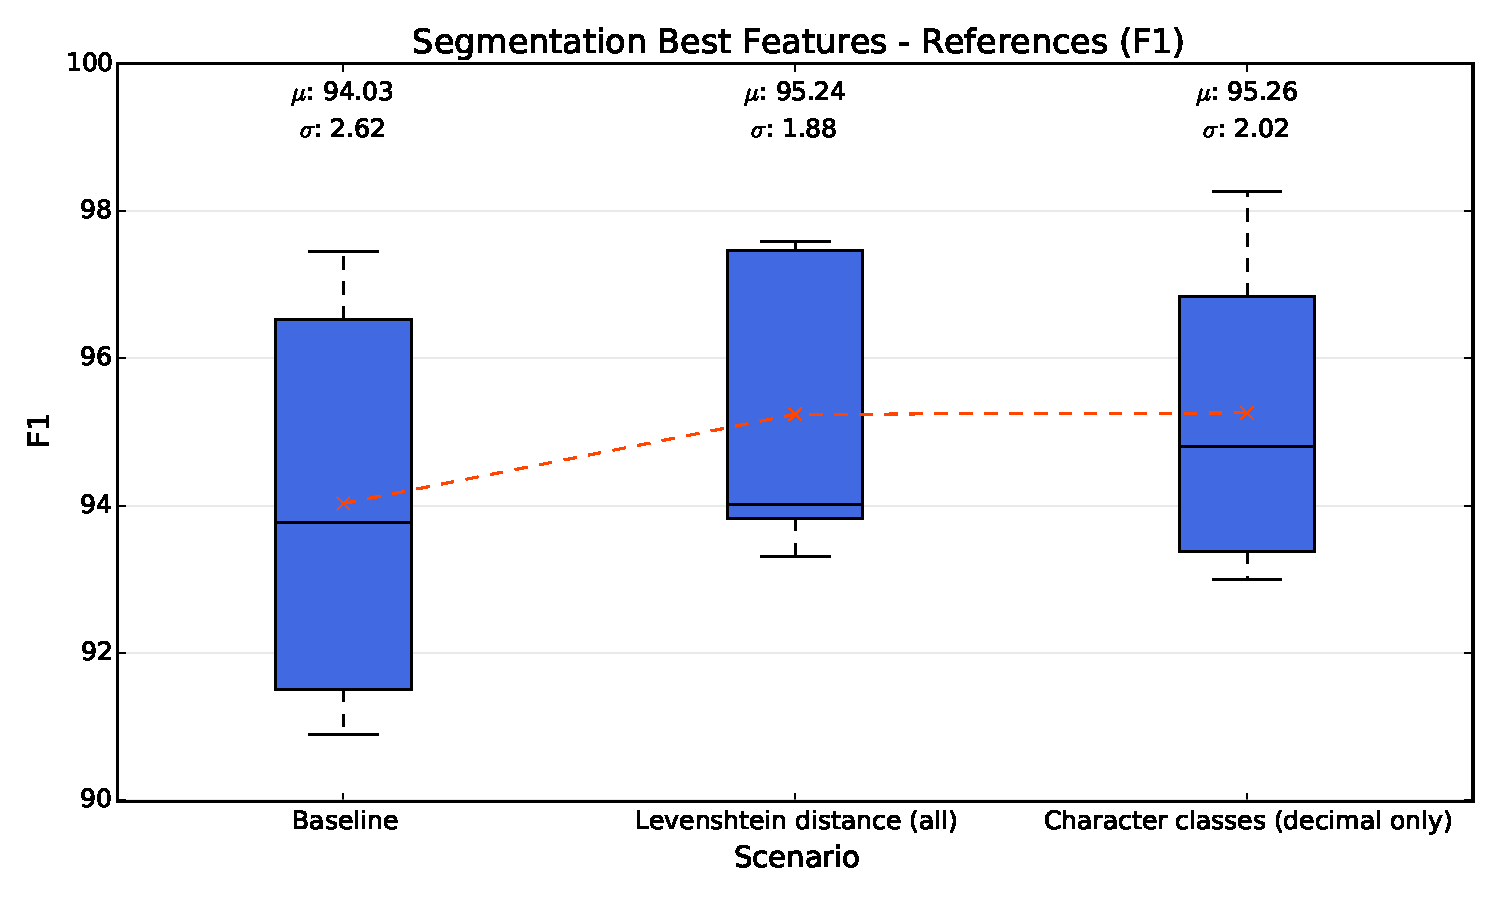
\includegraphics[width=5.5in]{Figures/references.pdf}
\caption{}
\label{fig:references}
\end{figure}

